\begin{figure}[H]
\centering
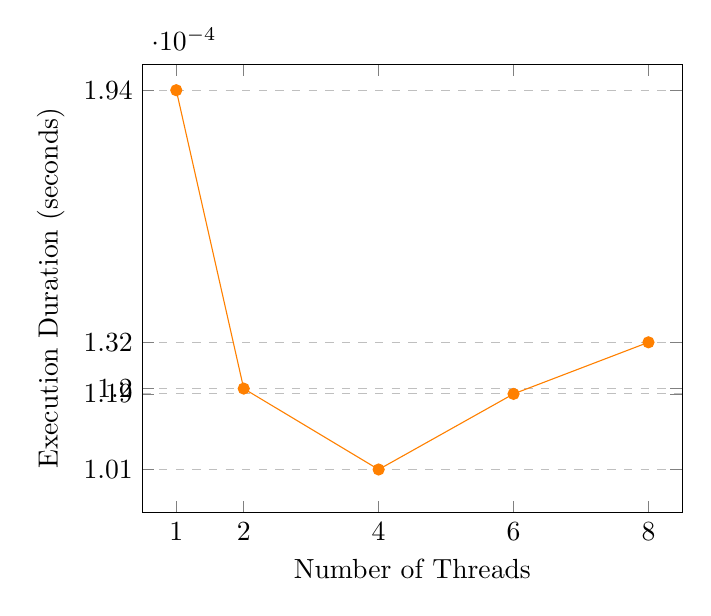
\begin{tikzpicture}
\begin{axis}[
    xlabel={Number of Threads},
    ylabel={Execution Duration (seconds)},
    xmin=0.5, xmax=8.5,
    ymin=0.00009, ymax=0.0002,
    xtick={1, 2, 4, 6, 8},
    ytick={0.0001936180000000,   0.0001204070000000,   0.0001005550000000,   0.0001191040000000,   0.0001317600000000},
    ymajorgrids=true,
    grid style=dashed,
]
\addplot[
    color=orange,
    mark=*,
    ]
    coordinates {
    (1, 0.0001936180000000) (2,0.0001204070000000) (4,0.0001005550000000) (6,0.0001191040000000) (8,0.0001317600000000)
    };

\end{axis}
\end{tikzpicture}
\caption{Execution Duration vs. Number of Threads for Hepta}
\label{fig:hepta}
\end{figure}